\chapter{Iterative Polynomial Space Solution}

This paper now introduces the iterative polynomial space solution to enumerating all minimal hypergraph traversals. First the depth control is used to expand the tree to the leaf (all hyperedges) and stores the next nodes to be processed later. Each node is then removed and processed, if the node is a leaf then the minimal transversal is visited, if the node is not a leaf then generate new children to process. Before adding the new work items to the queue, each of the new transversals must be appropriate. The implementation of an appropriate work item is introduced later. If no children are generated then this minimal transversal does not have any children after the next edge. 

\subsection{Define: Partial hypergraph transversal stack frame}
The previous definition of a partial hypergraph transversal does not take into account the additional list of generalized variables (odometers) needed for the function $IsAppropriate$.
A partial transversal stack frame $PTSF = (Transversals,Negations)$ is a collection where $Transversals$ is a list of generalized variables (odometers) as per the previous defintion with the additional $Negations$ as a list of generalized variables (odometers) for the function $IsAppropriate$.\\



\newpage
\section{Generate Next Depth}
This is a figure of the partial transversals enumerated while traversing the hypergraph $\{\{1,2,3\},\{3,4,5\},\{1,5\},\{2,5\}\}$. Each vertical column represents a generalized variable. Variables left of the plus $+$ sign are partial hypergraph transversals, variables in the center are the new hyperedge being encounter. Variables to the left of the minus $-$ sign are part of the negation list used for determining appropriate nodes to add. The leaf nodes are terminal results, they do not encounter a new hyperedge.\\

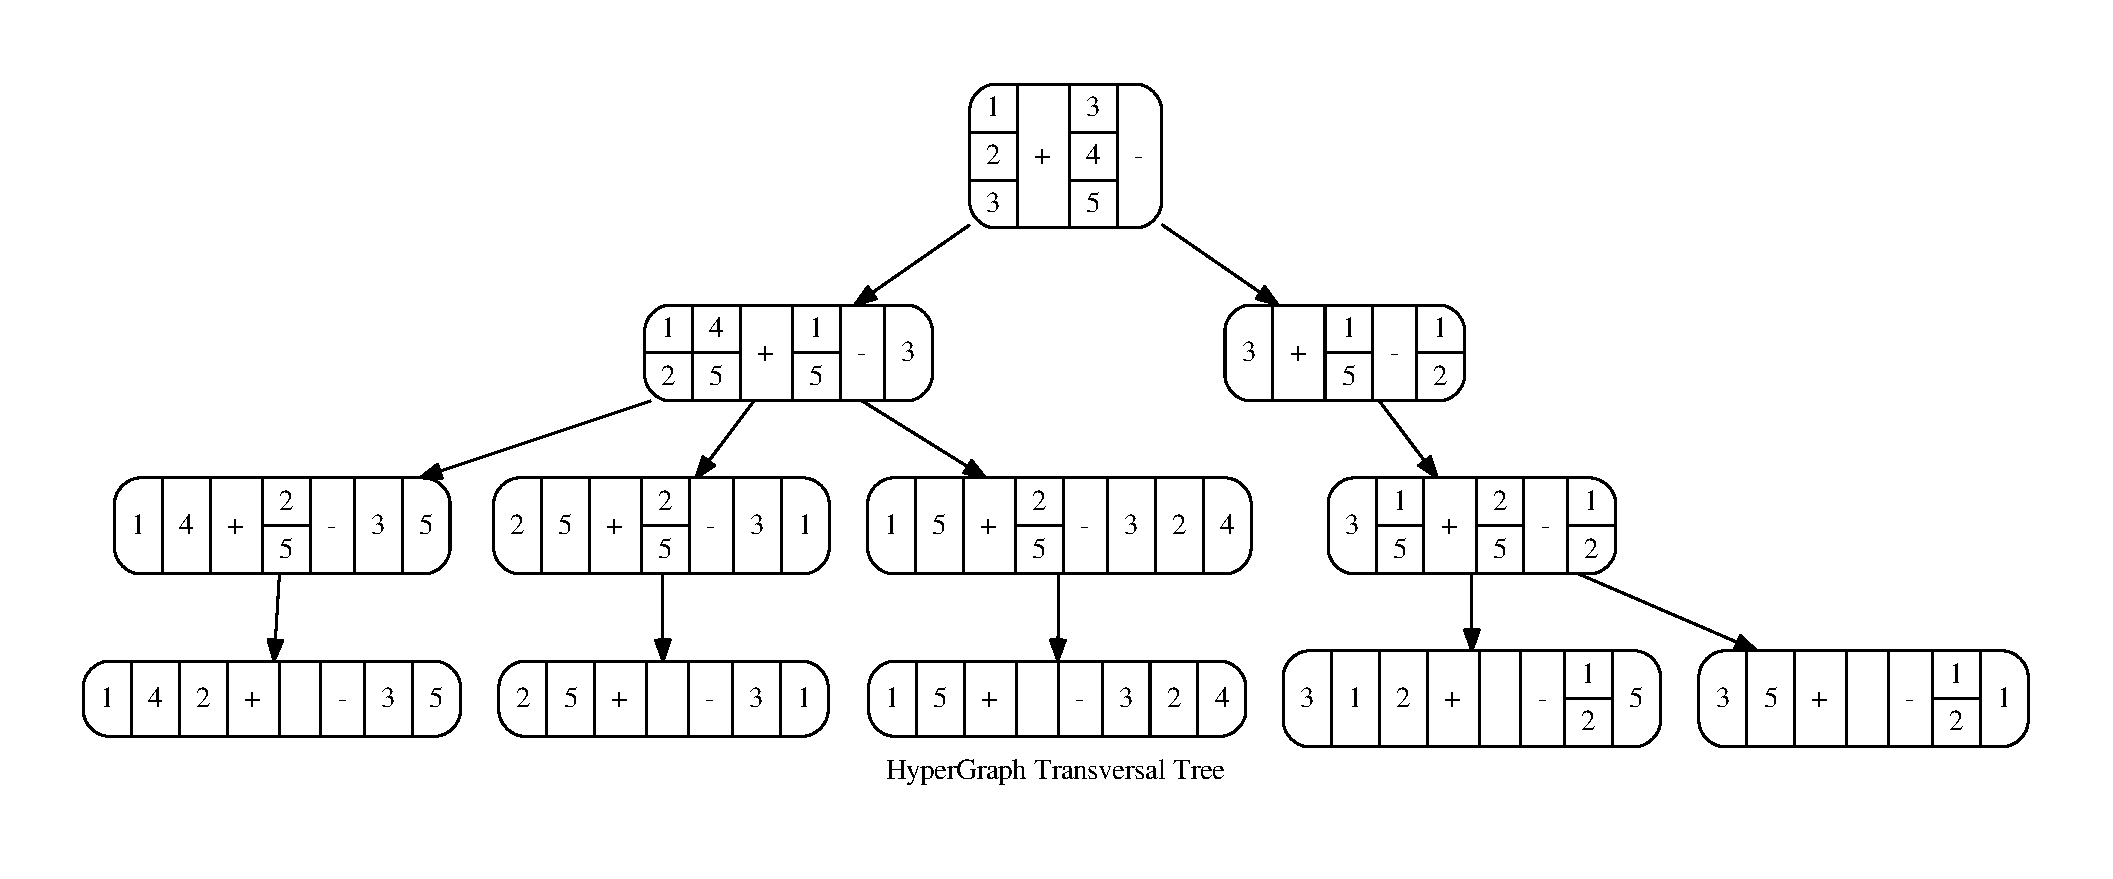
\includegraphics[scale=.4]{Paper.pdf}

\begin{algorithm}
	\caption{GenerateNextDepth}\label{GenerateNextDepth}
	\begin{algorithmic}[1]
		\Function{$GenerateNextDepth(HSF,edge)$}{}
		\State $new\_frame \gets \emptyset $ // hypergraph stack frame
		\State $return\_value \gets \emptyset $  // list of hypergraph stack frames.
		\State $result \gets IntersectTransversalWithEdge(HSF.Transversals,edge)$
		\If {$result.Gammas.size()==0$} 
		\State $new\_frame \gets HSF$ 
		\If {$result.Betas.size()>0$} 
		\ForAll {$\{b,i\} \in result.Beta$}
		\State $new\_frame.push(b)$    
		\EndFor
		\Else
		\State $new\_frame.push(edge)$ 
		\EndIf
		\If {$IsAppropriate(new\_frame,edge)$}
		\State $return\_value.push(new\_frame)$
		\EndIf
		\Else
		
		\ForAll {$list\_of\_bool \in Gen2expNtruefalse(result.Gammas.size()) $ }
			\State $new\_frame.Transversals \gets result.Alphas$
			\State $new\_frame.Negations \gets HSF.Negations$ 
			\ForAll {$\{tf,j\} \in list\_of\_bool$}
				\State $gamma \gets result.Gammas[j]$
				\If {$tf[j]=false$}
					\State $new\_frame.Transversals.push(gamma.XMinusY)$
					\State $new\_frame.Negations.push(gamma.XIntersectY)$
				\Else
					\State $new\_frame.Transversals.push(gamma.XIntersectY)$
				\EndIf
	
			\EndFor
			\If {$IsAllTrue(tf) = true $}
				\If {$result.new\_alpha.size()>0$}
				\State $new\_frame.Transversals.push(result.new\_alpha)$
				\EndIf
			\Else 
				\ForAll {$beta \in result.Betas$}
				\State $new\_frame.Transverals.push(beta)$
				\EndFor 
				\If {$IsAllFalse(tf)= true$}
				\ForAll {$gamma \in result.Gammas$}
				\State $new\_frame.Negations.push(gamma.XMinusY)$
				\EndFor 
				\EndIf
			
			\EndIf
		\If {$IsAppropriate(new\_frame,edge)=true$}
		\State $returnValue.push(new\_frame)$
		\State $new\_frame \gets \emptyset$
		\EndIf
		
		\EndFor
		\EndIf
		\State \Return $return\_value$
		\EndFunction
	\end{algorithmic}
\end{algorithm}



\newpage

Depth First N-Way Tree Control

\begin{algorithm}
	\caption{HypergraphTransversals}\label{HypergraphTransversals}
	\begin{algorithmic}[1]
		\Function{$HypergraphTransversals(H,CallbackFunc)$}{}
		\State $edge\_count \gets H.E.size()$
		\State $control\_stack \gets list(edge\_count)$ // list of stacks pre-sized.
		\State $HSF \gets \emptyset $ // current hypergraph stack frame
		\State $HSF.Transversals.push(edge)$
		\State $control \gets 0$ // depth control variable.
		\State $control\_stack[control].push(HSF)$ // load the process.
		\While {$control \geq 0$}
		\If {$control\_stack[control].size()=0$}
		\State $control \gets control-1$
		\Else
		\State $frame \gets control\_stack[control].pop()$
		\If {$control = edge\_count-1$}
		\State $CallbackFunc(frame.Transversals)$ // min transversal reached.
		\Else
		\State $control \gets control +1$
		\State $next\_edge \gets H.E[control]$
		\State $children \gets GenerateNextDepth(frame,next\_edge)$
		\ForAll {$\{c,i\} \in children$}
		\State $control\_stack[control].push(c)$ // next to be processed
		\EndFor 
		\EndIf
		\EndIf
		\EndWhile
		\EndFunction
	\end{algorithmic}
\end{algorithm}


\newpage

\section{IsAppropriate}

The following algorithm is used to determine if the new transversals 

\begin{algorithm}
	\caption{IsAppropriate}\label{IsAppropriate}
	\begin{algorithmic}[1]
		\Function{$IsAppropriate(HSF,edge)$}{}
		\State $list\_of\_new_traversals \gets \emptyset$
		\ForAll {$\{o,i\} \in HSF.Transversals$}
		\State $gv \gets o$
		\ForAll {$\{n,i\} \in HSF.Transversals$}
		\If {$DoesACoverB(n,gv)=true$}
		\State $gv \gets Minus(gv,n)$
		\EndIf
		\EndFor
		\If {$gv.size()>0$}
		\State $list\_of\_new_traversals.push(gv)$
		\EndIf
		\EndFor
		\If {$DoesAnyHitA(list\_of\_new_traversals ,edge)=false$}
		\State \Return $false$
		\EndIf
		\State \Return $true$
		\EndFunction
	\end{algorithmic}
\end{algorithm}